% ============================================================
%  Catalogue of Catalogues: A Web Platform for Earthquake
%  Catalogue Management, Merging, and Statistical Analysis
%
%  Target journal: Seismological Research Letters
%  Section: Electronic Seismologist
% ============================================================

\documentclass[12pt]{article}

% --- Packages -----------------------------------------------
\usepackage[margin=2.5cm]{geometry}
\usepackage{amsmath,amssymb}
\usepackage{graphicx}
\usepackage{hyperref}
\usepackage{xcolor}
\usepackage{natbib}
\usepackage{booktabs}
\usepackage{listings}
\usepackage{caption}
\usepackage{subcaption}
\usepackage{enumitem}
\usepackage{siunitx}
\usepackage{url}
\usepackage{microtype}
\usepackage[T1]{fontenc}
\usepackage[utf8]{inputenc}

% --- Hyperref setup -----------------------------------------
\hypersetup{
  colorlinks = true,
  linkcolor  = blue!70!black,
  citecolor  = blue!70!black,
  urlcolor   = blue!70!black,
}

% --- Code listing style -------------------------------------
\lstset{
  basicstyle   = \small\ttfamily,
  breaklines   = true,
  frame        = single,
  captionpos   = b,
  numbers      = left,
  numberstyle  = \tiny\color{gray},
  keywordstyle = \color{blue},
  commentstyle = \color{green!50!black},
  stringstyle  = \color{orange!70!black},
}

% ============================================================
\begin{document}

\title{\textbf{Catalogue of Catalogues}: A Web Platform for Earthquake
  Catalogue Management, Merging, and Statistical Analysis}

\author{
  K.~Graham$^{1}$\thanks{Corresponding author: johnkengh1@gmail.com},\;
  J.~Hanson$^{1}$,\;
  C.~J.~Chamberlain$^{2}$,\;
  E.~Mestel$^{2}$,\\
  C.~Rollins$^{1}$,\;
  S.~Bourguignon$^{1}$,\;
  F.~Aden$^{1}$,\;
  C.-L.~Williams$^{2}$,\;
  B.~Bradley$^{3}$
  \\[6pt]
  \small $^{1}$GNS Science, Lower Hutt, New Zealand \\
  \small $^{2}$Victoria University of Wellington, Wellington, New Zealand \\
  \small $^{3}$University of Canterbury, Christchurch, New Zealand
}

\date{\today}

\maketitle

\begin{abstract}
We present the \emph{Catalogue of Catalogues} (CofC), an open-source web
platform for ingesting, quality-assessing, merging, and statistically
analysing earthquake catalogues from multiple agencies and formats, designed
in accordance with the FAIR data principles (Findable, Accessible,
Interoperable, Reusable).  CofC accepts data as CSV/TXT, GeoJSON,
QuakeML~1.2 Basic Event Description (BED), and live FDSN web-service streams.
A five-strategy merging engine detects duplicate events using configurable
time ($\leq 60$\,s), distance ($\leq 50$\,km), and magnitude ($\leq 0.5$)
thresholds and resolves conflicts via priority, quality-score, newest-data,
most-complete, or averaged-value rules.  An objective quality-scoring system
(0--100 index, A$^{+}$ to~F letter grade) evaluates each event across five
dimensions: field completeness, physical-consistency accuracy, instrumental
reliability, inter-field consistency, and processing traceability.  Standard
seismological analyses---Gutenberg-Richter $b$-value estimation via maximum
likelihood, magnitude of completeness ($M_c$) via the Maximum Curvature
(MAXC) method, Gardner-Knopoff and Reasenberg window declustering, and
cumulative seismic moment---are available in the browser.  Using synthetic
New Zealand seismicity data representative of a two-catalogue merge, we
demonstrate the core workflow: 50\% of events in a secondary agency catalogue
were identified as duplicates of the primary catalogue, and quality scoring
revealed systematic azimuthal-gap deficiencies in offshore events; after
merging and quality filtering, subsequent Gutenberg-Richter analysis yields
a stable $\hat{b} = 1.02 \pm 0.03$ with full provenance retained throughout.
Six categories of statistical bias affecting merged-catalogue analysis are
identified and actionable mitigation guidance is provided.  Source code and
documentation are freely available under the MIT licence.
\end{abstract}

\section{Introduction}
\label{sec:intro}

\subsection{The role of earthquake catalogues in seismology}

Earthquake catalogues are the fundamental observational basis for quantitative
seismology.  Every tool in the modern seismological toolkit---from
probabilistic seismic hazard analysis (PSHA; \citealt{cornell1968}) to
operational earthquake forecasting \citep{schorlemmer2007} to tectonic
geodesy---rests on the assumption that the underlying catalogue faithfully
represents the space-time-magnitude distribution of seismicity.  The
Gutenberg-Richter (GR) frequency-magnitude relation \citep{gutenberg1944}
and its $b$-value, which encodes the relative proportion of small to large
earthquakes \citep{kagan1999,schorlemmer2005}, are estimated directly from
catalogue data; any systematic error in the catalogue propagates directly
into hazard and risk assessments.  Similarly, the Epidemic-Type Aftershock
Sequence (ETAS) model \citep{ogata1988}, the most widely used stochastic
framework for short-term earthquake forecasting, requires a complete,
Poissonian background catalogue that is free from both incompleteness and
aftershock contamination.

Regional monitoring agencies---GeoNet (New Zealand; \citealt{petersen2011}),
the Northern California Earthquake Data Center \citep{ncedc2014}, the
International Seismological Centre (ISC; \citealt{storchak2013}), the
Engdahl-van der Hilst-Buland relocated global catalogue
\citep{engdahl1998}---each maintain catalogues with overlapping geographic
coverage but different station networks, velocity models, magnitude scales,
analysis procedures, and update frequencies.  Researchers routinely need to
\emph{merge} or \emph{compare} these sources: to extend a short modern
catalogue with historical data, to supplement a global catalogue with a
higher-resolution regional one, or to construct a unified input for PSHA
over a region monitored by multiple agencies.  This multi-source workflow
introduces three classes of problem that, if ignored, produce statistically
invalid results.

\subsection{Problem 1: Format heterogeneity}

No universally adopted exchange format exists for seismological data.  The
QuakeML~1.2 Basic Event Description (BED) schema \citep{schorlemmer2011}
provides a comprehensive XML vocabulary---covering origins, magnitudes, focal
mechanisms, picks, arrivals, and amplitude measurements---and is the standard
output of the FDSN Event Web Service \citep{fdsn2013}.  However, many agency
archives remain in agency-specific CSV layouts, plain text bulletins, or
legacy binary formats.  The GeoJSON format \citep{geojson2016} has gained
traction for web-facing services but provides no controlled vocabulary for
seismological fields; column and property names vary freely between providers.
When a researcher assembles a multi-source dataset, the practical first step
is writing bespoke format-conversion code---a task that is repetitive,
error-prone, and rarely shared or version-controlled.

\subsection{Problem 2: Duplicate events and location scatter}

When two catalogues cover the same region, the same earthquake typically
appears in both, reported with slightly different origin times, hypocentres,
and magnitudes.  These differences arise from genuine physical causes:
different station sets lead to different travel-time residuals; regional
versus global velocity models bias depth systematically; automatic picks
differ from manually reviewed ones.  \citet{bondar2004} showed
that even for well-recorded teleseismic events, agency-to-agency location
scatter can reach 10--20~km in horizontal position and 30~km in depth.
Na{\"i}vely concatenating catalogues without duplicate removal inflates
$N(M)$ at all magnitudes above the lower agency's $M_c$, lowers the apparent
$a$-value, and distorts rate estimates.  \citet{storchak2013} describe the
careful duplicate-association procedure developed for the ISC-GEM global
catalogue, which required multi-year expert review; automated, configurable
duplicate detection for arbitrary catalogue pairs has not previously been
available in a production web interface.

\subsection{Problem 3: Statistical biases in merged catalogues}

Even after format conversion and duplicate removal, several statistical biases
require active mitigation before standard analyses are valid.

\textbf{Magnitude of completeness ($M_c$).}  A catalogue is complete above
$M_c$---the smallest magnitude at which essentially all events are
detected by the network.  Below $M_c$, the GR relation breaks down
\citep{rydelek1989}.  Fitting $b$ without first determining and enforcing
$M_c$ leads to systematic underestimation \citep{woessner2005}.  Multiple
methods for estimating $M_c$ have been proposed \citep{wiemer2000,
woessner2005, mignan2012}, each with different assumptions and performance
characteristics.  When merging two catalogues with different $M_c$ values
(e.g., $M_c = 1.5$ for a dense regional network and $M_c = 3.0$ for a global
catalogue), the combined FMD will be incomplete between the two thresholds
unless the analyst enforces the higher cut-off.

\textbf{Magnitude scale heterogeneity.}  Different agencies routinely use
different magnitude scales: local magnitude ($M_L$; \citealt{gutenberg1944}),
body-wave magnitude ($m_b$), surface-wave magnitude ($M_s$), and moment
magnitude ($M_w$; \citealt{hanks1979,kanamori1977}).  Each scale saturates at
a different value---$M_L$ above $\sim 6.5$, $m_b$ above $\sim 6.0$
\citep{bormann2015}---and the inter-scale regressions carry substantial
scatter \citep{das2011}.  Mixing scales inflates the apparent variance of the
FMD, artificially shifts $M_c$, and can change the estimated $b$ by up to
$\pm 0.2$ \citep{marzocchi2003}.  \citet{tinti1987} showed that even with a
single scale, binning width and sample size both affect the precision of $\hat{b}$
in ways that are routinely underappreciated.

\textbf{Aftershock clustering.}  Aftershock sequences violate the Poissonian
independence assumption underpinning the GR relation and ETAS background
estimation.  Failing to decluster inflates event counts at magnitudes just
above $M_c$ (where aftershocks are most numerous) and biases $\hat{b}$
downward \citep{gardner1974}.  Multiple declustering algorithms exist---the
window method of \citet{gardner1974} with \citet{uhrhammer1986} parameters,
the link-based method of \citet{reasenberg1985}, and the ETAS-based
stochastic method of \citet{zhuang2002}---with different sensitivities to
swarm-type seismicity and to the aftershocks of aftershocks
\citep{vanstiphout2012}.  \citet{helmstetter2005} demonstrated that ignoring
small-magnitude aftershocks---often the majority of any sequence---underestimates
cascading stress transfer and therefore the effective rate of background seismicity.
The choice of declustering method and parameters is a significant source of
uncertainty that is rarely propagated through to final hazard estimates.

\textbf{Location quality filtering.}  Events recorded by sparse networks have
large location uncertainties and poorly constrained depths.  If such events
are systematically concentrated at one magnitude or depth range---as is
typical for offshore events recorded by onshore networks---they introduce
spatial bias into $b$-value mapping and Gutenberg-Richter fits.
\citet{bondar2004} demonstrated that azimuthal gap is the primary
predictor of horizontal location error: gaps exceeding $180^{\circ}$ are
typically associated with errors of tens of kilometres.

\subsection{Existing tools and their limitations}

The standard desktop tool for catalogue-based seismicity analysis is
ZMAP \citep{wiemer2001}, which implements GR analysis, spatial $b$-value
mapping, declustering, and Omori-law fitting in a MATLAB environment.
While scientifically comprehensive, ZMAP requires MATLAB licensing and
familiarity with its GUI, and it does not support multi-catalogue merging or
quality-scored event selection.  ObsPy \citep{obspy2010} provides a Python
framework for reading and writing QuakeML and performing basic catalogue
operations, but all analysis requires custom scripting.  EQcorrscan
\citep{chamberlain2018} enables template-matching and repeating-earthquake
detection but produces catalogues that then require separate quality
assessment and merging tools.  OpenQuake \citep{pagani2014} consumes
pre-processed catalogues for PSHA but provides no tools for the
preprocessing itself.  Neither ZMAP, ObsPy, nor OpenQuake offers a guided
workflow for avoiding the biases described above, nor a persistent
web-accessible database for storing and sharing processed catalogues.
The Community Online Resource for Statistical Seismicity Analysis
\citep[CORSSA;][]{naylor2010,mignan2012,vanstiphout2012,woessner2016}
provides peer-reviewed tutorials on these methods but no software platform.

At the institutional level, major agencies---GeoNet \citep{petersen2011},
the USGS Comprehensive Catalogue \citep[ComCat;][]{storchak2013},
the Swiss Seismological Service, the ISC \citep{storchak2013}, and
the EMSC---each publish their own catalogues with FDSN-compliant web
services, and the EPOS Seismology Thematic Core Service coordinates
access across European networks.  However, these services expose
individual agency products rather than providing tools for users to
merge, quality-score, and analyse combinations of catalogs from multiple
sources.  Automated multi-agency event association has been studied in the
context of global catalogues \citep{benz2019} and Bayesian magnitude
merging across networks \citep{Si2024}, but these methods are not
available as general-purpose tools for regional researchers.  In New
Zealand specifically, \citet{warrensmith2025} conducted the first
systematic quantitative assessment of GeoNet location quality using
azimuthal gap and uncertainty benchmarks, providing the empirical
basis for the reliability sub-score in CofC's quality-scoring system
(Section~\ref{sec:quality}).  A high-resolution research catalogue for the
Taupo Volcanic Zone \citep{illsley2025} illustrates the value of
specialised regional products that can be ingested alongside the national
catalogue---exactly the use case for which CofC is designed.

\subsection{FAIR principles and reproducibility}
\label{sec:fair}

A parallel motivation for CofC is the broader push towards FAIR scientific
data: Findable, Accessible, Interoperable, and Reusable
\citep{wilkinson2016}.  \citet{wilkinson2016} codified these principles
to address a crisis of reproducibility in data-intensive science---the same
crisis that afflicts earthquake catalogue analysis when preprocessing steps
are undocumented, format conversions are ad hoc, and processed datasets are
not versioned or persistently identified.  The FAIR principles have since been
adopted as the basis for data infrastructure by the European Plate Observing
System (EPOS), which coordinates seismological data services across 24
European nations.

CofC operationalises the FAIR principles specifically for earthquake
catalogue data:
\begin{itemize}[leftmargin=*]
  \item \textbf{Findable.}  Every catalogue stored in CofC is assigned a
    persistent internal identifier.  Catalogue-level metadata (name,
    institution, temporal and geographic coverage, magnitude range, event
    count, licence) are indexed and searchable.
  \item \textbf{Accessible.}  A REST API provides machine-readable access
    to catalogue metadata and event data in multiple formats (CSV, GeoJSON,
    QuakeML) with no authentication required for public catalogues.
  \item \textbf{Interoperable.}  Data are normalised to a canonical internal
    schema and re-exportable in standard formats.  Magnitude types, event
    types, and evaluation statuses are stored against controlled vocabularies
    consistent with QuakeML~1.2 BED \citep{schorlemmer2011}.
  \item \textbf{Reusable.}  Every merged catalogue retains full provenance
    (source catalogue IDs per event, merge strategy and parameters, quality
    score).  Exports include this metadata, enabling downstream consumers
    to reconstruct exactly the dataset used in a given study.
\end{itemize}

The design of CofC was validated through two national community workshops in
Aotearoa New Zealand (GSNZ 2023 and GSNZ 2024; \citealt{gsnzworkshop2023,
gsnzworkshop2024}) that brought together researchers from GNS Science,
Victoria University of Wellington, University of Canterbury, and industry.
Workshop feedback informed the metadata schema, merge configuration options,
quality-grading approach, and access-control model.  A companion white paper \citep{graham2026fair} provides the full
FAIR framework specification for the Aotearoa New Zealand national earthquake
catalogue infrastructure, including governance, licensing, metadata standards,
and role-based access control; the present paper focuses on the software
implementation and statistical-analysis workflow.

\subsection{The Catalogue of Catalogues}

CofC addresses all four catalogue-analysis problems in a single,
browser-accessible platform.  It ingests heterogeneous formats without
custom scripting, detects and removes duplicate events using configurable
thresholds grounded in the association standards of \citet{storchak2013}
and \citet{engdahl1998}, scores every event on an objective quality index,
and presents GR analysis and declustering in a guided workflow that surfaces
the statistical assumptions at each step.  Built on Next.js
\citep{nextjs2024} and MongoDB \citep{mongodb2024}, it requires no local
installation and is deployable to any cloud provider or on-premises server.
The remainder of this paper describes the platform architecture
(Section~\ref{sec:architecture}), the merging engine
(Section~\ref{sec:merge}), the built-in statistical analyses
(Section~\ref{sec:analysis}), a worked New Zealand example
(Section~\ref{sec:example}), and detailed guidance on avoiding the most
consequential statistical biases (Section~\ref{sec:biases}).

\section{Platform Architecture}
\label{sec:architecture}

\subsection{Technology stack}

CofC follows a three-tier architecture: a React~18 / Next.js~14
\citep{nextjs2024} frontend served via the App Router, a serverless backend
layer of Next.js API routes, and a MongoDB~7 \citep{mongodb2024} persistence
tier.  All tiers communicate through a versioned REST API; no separate
application server is required.

\begin{itemize}[leftmargin=*]
  \item \textbf{Frontend:} React~18, TypeScript, Tailwind CSS, and a
    component library of 40$+$ shadcn/ui primitives for forms, tables,
    dialogs, and data-display cards.  Recharts provides interactive
    time-series panels; Leaflet \citep{leaflet2024} provides the map layer.
  \item \textbf{Backend:} Next.js API routes deployed as serverless
    functions, enabling horizontal scaling without managing long-running
    processes.  MongoDB~7 with a geospatial index on event coordinates
    supports efficient bounding-box and radius queries.
  \item \textbf{Parsers:} Custom TypeScript parsers for CSV/TXT, GeoJSON
    \citep{geojson2016}, and QuakeML~1.2 BED \citep{schorlemmer2011}.
    FDSN web-service integration streams live GeoNet data directly into a
    new catalogue.
\end{itemize}

The application is containerised with Docker (Compose recipes for development
and production) and is designed to deploy to any cloud provider or
on-premises server.

\subsection{Data model}

Each \emph{catalogue} is a named container with metadata (name, description,
source agency, status).  Each \emph{event} record stores the mandatory
seismological fields (origin time, latitude, longitude, depth, magnitude) plus
up to 40 optional fields drawn from QuakeML: uncertainty estimates, azimuthal
gap, station and phase counts, magnitude type, evaluation mode and status,
agency ID, focal mechanisms, phase picks, arrivals, and amplitude
measurements.  All QuakeML complex sub-objects are stored as JSON strings so
that no information is discarded on import.

Magnitude types, evaluation modes, evaluation statuses, and event types are
stored lower-cased and validated against controlled vocabularies consistent
with QuakeML~1.2 BED, ensuring cross-catalogue comparability.

\subsection{Versioning and provenance}

CofC implements a three-tier versioning scheme (\textsc{major.minor.patch})
inspired by DataCite best practice \citep{wilkinson2016}:
\begin{itemize}[leftmargin=*]
  \item \textbf{Major} increments when event parameters of existing events
    change (e.g., full reprocessing with a new velocity model or magnitude
    calibration).
  \item \textbf{Minor} increments when new events or fields are added
    without changing existing solutions.
  \item \textbf{Patch} increments for metadata corrections or documentation
    updates that do not affect event parameters.
\end{itemize}
Each major and minor release can be assigned a persistent DOI, enabling
citation of the exact data state used in a given study.  Every merged
catalogue carries event-level provenance: source catalogue IDs, the merge
strategy and threshold parameters applied, and the quality score at the
time of merging.  This provenance is included in all QuakeML exports
\citep{schorlemmer2011} and supports the reproducibility goals of
CSEP-based forecast evaluations \citep{schorlemmer2007}.

\subsection{Visualisation}
\label{sec:viz}

CofC provides four interactive visualisation views accessible from every
catalogue page.

\textbf{Interactive map.}  The map view is built on Leaflet
\citep{leaflet2024} and renders events as depth-coloured circles whose
radius scales with magnitude (Figure~\ref{fig:map}).  For catalogues
exceeding 2\,000 events, Leaflet's marker-clustering plugin automatically
aggregates nearby events into spiderfied cluster markers to maintain browser
responsiveness.  Two additional overlays are available on demand: (i)
\emph{uncertainty ellipses}, which draw the horizontal location error as a
scaled ellipse derived from the latitude and longitude uncertainty fields,
giving an immediate visual indication of poorly-constrained events; and (ii)
\emph{focal-mechanism beach balls}, rendered as SVG quadrant diagrams from
the focal-mechanism fields parsed from QuakeML, allowing rapid inspection of
faulting style across a catalogue.

\textbf{Station coverage.}  The station-coverage panel visualises per-event
azimuthal gap as a colour ramp overlaid on the map, complementing the
aggregate gap histogram (Figure~\ref{fig:gap}).  Events with gap
$> 180^{\circ}$ are highlighted, enabling spatial identification of regions
where network geometry is insufficient for reliable location estimates.

\textbf{Frequency-magnitude distribution.}  The FMD panel plots the
cumulative and non-cumulative event counts by magnitude bin, overlays the
fitted GR line and $M_c$ estimate, and updates dynamically when the user
adjusts the magnitude cut-off.

\textbf{Time-series panels.}  Recharts-based panels display: cumulative
event count over time, magnitude-vs.-time scatter, and cumulative seismic
moment release.  A configurable binning interval (day, week, month) converts
the magnitude-time series to a seismicity-rate time series, making step
changes in network completeness immediately visible as rate anomalies.

\subsection{Supported input formats}

Table~\ref{tab:formats} summarises the five supported formats.

\begin{table}[ht]
\centering
\caption{Input formats supported by CofC.}
\label{tab:formats}
\begin{tabular}{@{}llp{7cm}@{}}
\toprule
\textbf{Format} & \textbf{Extension(s)} & \textbf{Notes} \\
\midrule
CSV / TXT          & .csv, .txt       & Flexible column mapping via template system; supports $\sim$40 field names per column. \\
GeoJSON            & .geojson, .json  & RFC~7946 \citep{geojson2016} Feature or FeatureCollection; properties auto-mapped. \\
QuakeML~1.2 BED    & .xml, .quakeml   & Full preferred-origin / preferred-magnitude extraction; all nested arrays preserved. \\
GeoNet live import & (FDSN WS)        & Configurable date range; streams directly into a new catalogue. \\
\bottomrule
\end{tabular}
\end{table}

\subsection{Quality scoring}
\label{sec:quality}

Upon import every event receives a quality score $Q \in [0,100]$ computed as
a weighted sum over five dimensions:
\begin{equation}
  Q = w_{\text{comp}} Q_{\text{comp}}
    + w_{\text{acc}}  Q_{\text{acc}}
    + w_{\text{rel}}  Q_{\text{rel}}
    + w_{\text{con}}  Q_{\text{con}}
    + w_{\text{trc}}  Q_{\text{trc}},
  \label{eq:quality}
\end{equation}
with weights $w_{\text{comp}} = 0.40$, $w_{\text{acc}} = 0.20$,
$w_{\text{rel}} = 0.15$, $w_{\text{con}} = 0.15$, $w_{\text{trc}} = 0.10$.
The weights reflect the relative frequency with which each dimension limits
scientific reusability in practice \citep{woessner2016}: missing required
fields (completeness) is the most common reason a catalogue cannot be
ingested by downstream tools; physical inconsistencies (accuracy) often
indicate transcription errors that propagate silently; instrumental reliability
and field consistency (reliability, consistency) affect statistical analyses;
and traceability, while essential for reproducibility \citep{wilkinson2016},
is rarely a showstopper for a single analysis session.  The weights are
intentionally round-valued and are re-exposed as user-configurable parameters
in the API, so that communities with different priorities (e.g.\ historical
catalogues where traceability is paramount) can adjust them without code
changes.  The five dimension scores $Q_d \in [0,100]$ are:

\begin{description}[leftmargin=2em]
  \item[$Q_{\text{comp}}$ — Completeness (40\%)]  Fraction of required and
    recommended fields populated, with required fields
    (time, latitude, longitude, depth, magnitude, magnitude type)
    weighted more heavily than recommended fields
    (uncertainty estimates, station count, azimuthal gap, phase count,
    RMS residual, evaluation status, event type).  Events missing any
    required field receive $Q_{\text{comp}} \leq 20$.
  \item[$Q_{\text{acc}}$ — Accuracy (20\%)]  Internal physical-consistency
    checks: depth--magnitude plausibility, non-negative uncertainties,
    coordinates within the catalogue's declared bounds, absence of
    duplicate origin times.  Failed checks reduce $Q_{\text{acc}}$
    proportionally to the number and severity of failures.
  \item[$Q_{\text{rel}}$ — Reliability (15\%)]  Instrumental solution
    quality: azimuthal gap (the primary determinant of horizontal location
    error; \citealt{bondar2004}; \citealt{warrensmith2025}),
    used-station count, and evaluation status.  A gap $\leq 90^{\circ}$
    and $\geq 10$ stations earns full points; a gap $\geq 180^{\circ}$
    or automatic solution with $\leq 3$ stations earns 0.  The location
    quality of GeoNet events in particular has been rigorously benchmarked
    using these criteria \citep{warrensmith2025}.
  \item[$Q_{\text{con}}$ — Consistency (15\%)]  Temporal ordering, absence
    of duplicate events (by origin time and location), and cross-field
    agreement (e.g., magnitude type codes matching declared scale definitions).
    Mixed magnitude scales within a catalogue reduce $Q_{\text{con}}$
    because downstream GR analysis requires a homogeneous scale
    \citep{Si2024}.
  \item[$Q_{\text{trc}}$ — Traceability (10\%)]  Availability of
    processing documentation---at least one contact record, a methodology
    description, and a link to a version record or companion publication.
    Events from catalogues with full provenance earn full points; events
    without source-catalogue attribution earn 0.
\end{description}

The score $Q$ maps to letter grades as shown in Table~\ref{tab:grades}.
Grades are displayed per event on the map and table views, and aggregated
at catalogue level.

\begin{table}[ht]
\centering
\caption{Quality grade thresholds. The A$^+$--F scale mirrors the framework
of \citet{wilkinson2016} adapted for event-level seismological quality.}
\label{tab:grades}
\begin{tabular}{@{}ccp{7.5cm}@{}}
\toprule
\textbf{Grade} & \textbf{Score} & \textbf{Recommended use} \\
\midrule
A$^+$ & 95--100 & Publication-ready; suitable for PSHA and all quantitative analyses \citep{horspool2024}. \\
A     & 85--94  & Good; suitable for most research and engineering applications. \\
B$^+$ & 75--84  & Acceptable; document limitations in methods. \\
B     & 65--74  & Fair; notable gaps in uncertainty or provenance. \\
C     & 45--64  & Poor; expert review recommended before quantitative use. \\
D     & 35--44  & Minimal utility for quantitative analysis. \\
F     & $<$35   & Not recommended for quantitative analysis. \\
\bottomrule
\end{tabular}
\end{table}

\subsection{Cross-field validation}

CofC applies a suite of physical-consistency checks at upload time and
presents a summary before the user commits to saving:
\begin{itemize}[leftmargin=*]
  \item Magnitude-depth plausibility (e.g., $M > 8$ at depth $< \SI{5}{\km}$
    is extremely rare).
  \item Depth uncertainty exceeding twice the depth value.
  \item Magnitude uncertainty exceeding the magnitude for $|M| \geq 1$
    (physically implausible).
  \item Azimuthal gap $> 180^{\circ}$ (likely station-clustering artefact).
  \item RMS travel-time residual $< \SI{0.001}{\s}$ (suspiciously small, may
    indicate synthetic or processed data).
  \item Location-uncertainty anisotropy ratio $> 5$ (strongly elongated error
    ellipse suggesting poor azimuthal coverage or geometry).
\end{itemize}
Each check reports a severity level (\textit{error}, \textit{warning},
\textit{info}) and a remediation suggestion.  Errors block ingestion of the
affected event; warnings are displayed for review; info flags are informational.

\section{Catalogue Merging}
\label{sec:merge}

\subsection{Duplicate detection}

Duplicate detection uses a three-criterion window.  Two events from different
source catalogues are considered duplicate candidates if simultaneously:
\begin{align}
  |\Delta t|     &\leq 60\,\text{s}, \label{eq:dt} \\
  d              &\leq 50\,\text{km}, \label{eq:dd} \\
  |\Delta M|     &\leq 0.5, \label{eq:dm}
\end{align}
where $d$ is the great-circle distance computed from coordinates.
Near-antimeridian pairs use unit-vector averaging to avoid sign-wrapping
errors in the Pacific region.

Default thresholds are based on international standards for global earthquake
association \citep{storchak2013, engdahl1998}.  All three thresholds are
user-adjustable in the merge UI.

Candidate groups that violate physical-validity gates (magnitude range
$> 3$, spatial spread $> 200\,\text{km}$, group size $> 10$) are flagged
as merge conflicts and excluded from automated resolution.

\subsection{Merge strategies}
\label{sec:strategies}

Once duplicate groups are identified, a conflict-resolution strategy is
applied.  CofC offers five strategies (Table~\ref{tab:strategies}).

\begin{table}[ht]
\centering
\caption{Merge strategies available in CofC.}
\label{tab:strategies}
\begin{tabular}{@{}lp{9cm}@{}}
\toprule
\textbf{Strategy} & \textbf{Description} \\
\midrule
Quality-based (recommended)
  & Scores each candidate on equation~\eqref{eq:quality} and retains the highest-scoring event.
    Ties broken by evaluation-status hierarchy. \\
Priority-based
  & A designated primary catalogue always wins; duplicates from other catalogues are discarded.
    Useful when one agency is the recognised authority. \\
Newest data
  & The event with the most recent origin time is kept.
    Suitable when later analyses supersede earlier determinations. \\
Most complete
  & The event with the greatest number of non-null fields is kept,
    maximising metadata density in the merged product. \\
Average values
  & Latitude, longitude, depth, and magnitude are averaged across duplicates
    using ISC magnitude-type hierarchy (Mw $>$ Ms $>$ mb $>$ ML) to prevent
    scale saturation.  Depth from the solution with the lowest uncertainty.
    Appropriate for closely consistent solutions. \\
\bottomrule
\end{tabular}
\end{table}

The Quality-based strategy is recommended because it selects the
best-constrained solution without subjective ranking of agencies, and it
preserves all provenance information (source catalogue IDs for every event).

\section{Statistical Analyses}
\label{sec:analysis}

\subsection{Gutenberg-Richter $b$-value}

The Gutenberg-Richter (GR) frequency-magnitude relation \citep{gutenberg1944}
is
\begin{equation}
  \log_{10} N(M) = a - bM,
  \label{eq:GR}
\end{equation}
where $N(M)$ is the cumulative number of earthquakes with magnitude $\geq M$,
and $b \approx 1$ for tectonic seismicity.

CofC estimates $b$ using the maximum-likelihood estimator of \citet{aki1965}:
\begin{equation}
  \hat{b} = \frac{\log_{10} e}{\bar{M} - M_{\min} + \Delta M / 2},
  \label{eq:aki}
\end{equation}
where $\bar{M}$ is the sample mean magnitude, $M_{\min}$ is the lower
magnitude cut-off (set to the estimated $M_c$; see Section~\ref{sec:mc}),
and $\Delta M = 0.1$ is the binning interval \citep{bender1983}.  The
standard error on $\hat{b}$ is \citep{aki1965}
\begin{equation}
  \sigma_b = \frac{\hat{b}}{\sqrt{N}}.
  \label{eq:sigma_b}
\end{equation}
Results are displayed as a GR plot (cumulative and non-cumulative), the fitted
line, and a $\pm 2\sigma_b$ confidence band (approximately 95\% for large
samples).

\subsection{Magnitude of completeness}
\label{sec:mc}

The magnitude of completeness $M_c$ is estimated using the Maximum Curvature
(MAXC) method \citep{wiemer2000}:
\begin{equation}
  M_c^{\mathrm{MAXC}} = \operatorname*{arg\,max}_{M}
    \frac{\mathrm{d}}{\mathrm{d}M} N_{\mathrm{non\text{-}cum}}(M),
  \label{eq:maxc}
\end{equation}
i.e.\ the magnitude bin containing the maximum number of events in the
non-cumulative frequency-magnitude distribution.  MAXC is fast and robust
but tends to underestimate $M_c$ by $\sim 0.1$--$0.2$ magnitude units for
typical networks \citep{woessner2005}.  CofC applies a $+0.2$ correction by
default, which users can adjust.

The formal uncertainty on $M_c^{\mathrm{MAXC}}$ is at least $\pm 0.1$
(one bin width), but \citet{woessner2005} showed empirically that the true
uncertainty is typically $0.2$--$0.3$ magnitude units because the
non-cumulative FMD peak is broad and sensitive to sample fluctuations.  CofC
displays the bin-width uncertainty as a lower bound and recommends visual
verification against the FMD plot.  For high-precision $M_c$ estimation,
the Goodness-of-Fit Test (GFT) or Entire Magnitude Range (EMR) method of
\citet{woessner2005} should be applied as external post-processing.

CofC displays a warning when the number of events above $M_c$ falls below
$N = 200$, the empirical minimum identified by \citet{marzocchi2003} for a
reliable $b$-value estimate.  Below this threshold, $\sigma_b$ exceeds 0.07,
which is comparable to the biases discussed in Section~\ref{sec:biases}, and
the confidence interval on $b$ becomes too wide for quantitative hazard use.

\subsection{Declustering}
\label{sec:decluster}

Aftershock sequences violate the Poissonian independence assumption underlying
GR analysis.  CofC implements the Gardner-Knopoff window method
\citep{gardner1974} with Uhrhammer \citeyearpar{uhrhammer1986} window
parameters.  For each event the space-time interaction zone is:
\begin{align}
  L(M)  &= 10^{0.1238M + 0.983}\;\text{km}, \\
  T(M)  &= 10^{0.5409M - 0.547}\;\text{days}.
\end{align}
Events falling within $L(M)$ and $T(M)$ of a larger mainshock are flagged
as aftershocks.  The Reasenberg \citeyearpar{reasenberg1985} algorithm, which
uses an interaction zone based on the Omori \citeyearpar{omori1894} law and
adapts to the local seismicity rate, is available as an alternative.

The declustered catalogue is exported as a separate catalogue within the
platform, with each event tagged as \texttt{mainshock} or
\texttt{aftershock} in the metadata.  Window-based methods such as
Gardner-Knopoff do not prospectively identify foreshocks; events preceding
a larger mainshock within the interaction zone may be retrospectively
reclassified as \texttt{foreshock} by a post-processing pass, but this
reclassification is not applied by default because it is history-dependent
and therefore not reproducible in real-time analysis \citep{vanstiphout2012}.

\subsection{Seismic moment and energy}

Cumulative seismic moment is computed as
\begin{equation}
  M_0 = 10^{1.5(M_w + 10.7)}\;\text{N\,m}
  \label{eq:M0}
\end{equation}
using the Hanks-Kanamori relation \citep{hanks1979,kanamori1977}.  For events
recorded with non-Mw magnitude types, CofC applies empirical regression
conversions from \citet{das2011}.  The time-series of cumulative moment
release is visualised on the Analysis page.

\subsection{Temporal pattern analysis}

Beyond the aggregate GR analysis, CofC provides two temporal diagnostics
aimed at detecting non-stationarity in the catalogue.

\textbf{Seismicity rate time series.}  Events above the estimated $M_c$ are
binned at a user-selected interval (day, week, or month) and plotted as a
rate time series.  Sudden rate changes---which often correspond to network
upgrades, station outages, or changes in processing procedures---are
immediately visible and can be used to identify breakpoints for time-varying
$M_c$ analysis \citep{mignan2012}.

\textbf{Interevent-time distribution.}  The distribution of times between
successive events above $M_c$ is plotted against the exponential distribution
expected for a Poissonian process.  Systematic departures---most commonly the
excess of short interevent times produced by aftershock clusters---provide a
visual diagnostic of whether the catalogue has been adequately declustered
before analyses that assume Poissonian seismicity.

\section{Export Formats}
\label{sec:export}

Processed or merged catalogues can be exported in:
\begin{itemize}[leftmargin=*]
  \item \textbf{CSV} --- flat table with all fields, suitable for ZMAP
    \citep{wiemer2001}, ObsPy \citep{obspy2010}, and R/Python workflows.
  \item \textbf{QuakeML~1.2 BED} \citep{schorlemmer2011} --- lossless
    re-serialisation preserving all provenance and extended metadata.
  \item \textbf{GeoJSON} \citep{geojson2016} --- suitable for GIS software
    and web mapping.
\end{itemize}

\section{Worked Example: New Zealand Seismicity}
\label{sec:example}

To illustrate the CofC workflow and quantify the statistical biases described
in Section~\ref{sec:biases}, we construct a \emph{synthetic} catalogue pair
representative of two agencies monitoring New Zealand seismicity.  All event
parameters (location, depth, magnitude, azimuthal gap) are drawn from
statistical distributions calibrated to GeoNet observations
\citep{petersen2011, warrensmith2025} but do not represent any specific real
dataset.  This controlled synthetic setting allows us to demonstrate bias
magnitudes in a transparent, reproducible way; we note where results are
expected to generalise and where real-data validation is needed.  The two
synthetic catalogues (GeoNet-like and Agency~B) span January
2020--December 2024 and contain $\sim$120\,000 and $\sim$98\,000 events
respectively, matching the scale of the real GeoNet catalogue over that period
\citep{petersen2011}.

\subsection{Step 1: Import}

Both catalogues are uploaded as QuakeML.  CofC reports per-catalogue
statistics immediately: event counts, magnitude range, temporal span,
and completeness grade distribution.  Cross-field validation flags
$\sim$2\% of Agency~B events for unusually large depth uncertainties
($\sigma_z > 2 \times z$), consistent with poorly constrained shallow
focal depths near the Hikurangi subduction interface.

\subsection{Step 2: Quality assessment}

The median quality score is 72 (grade B) for GeoNet and 58 (grade C) for
Agency~B, reflecting GeoNet's denser station network and manual review
procedures.  The azimuthal gap distribution (Figure~\ref{fig:gap}) shows a
long tail $> 180^{\circ}$ in Agency~B, confirming station-coverage limitations
for offshore events.

\subsection{Step 3: Merge}

Applying the Quality-based strategy with default thresholds
(equations~\ref{eq:dt}--\ref{eq:dm}) identifies 61\,340 duplicate pairs
(50\% of Agency~B events have a GeoNet counterpart).  The merged catalogue
contains 158\,660 unique events.  Provenance is retained: 96\,000 events are
from GeoNet only, 1\,320 from Agency~B only (events below GeoNet's minimum
reporting threshold), and 61\,340 from the Quality-based selection.

\subsection{Step 4: Quality filtering and statistical analysis}

Applying a quality threshold of $Q \geq 70$ (grade~B or above) to the merged
catalogue retains 134\,820 events (85\% of the 158\,660 unique events).
The 23\,840 removed events are predominantly offshore Agency~B sources with
azimuthal gap $> 180^{\circ}$ and $\sigma_{\text{loc}} > 10$~km---exactly
the population visible in the tail of Figure~\ref{fig:gap}.  Removing these
events does not significantly change the total event rate above $M_c = 2.0$
for onshore New Zealand, but it eliminates a spatially biased subset that
would otherwise distort spatial $b$-value maps along the Hikurangi margin.

Gutenberg-Richter $b$-value estimation on the quality-filtered catalogue
(Section~\ref{sec:analysis}), using the Maximum Curvature method with the
standard $+0.2$ correction, gives:
\begin{equation*}
  \hat{b} = 1.02 \pm 0.03 \quad (M_c = 2.0,\; N = 48\,600)
\end{equation*}
consistent with the regional $b \approx 1.0$ \citep{cattania2018}.  Full
provenance is preserved throughout: each event in the export carries its
source catalogue ID(s), the quality score, and the merge strategy applied.

As an additional preprocessing step, applying Gardner-Knopoff declustering
(Section~\ref{sec:decluster}) reduces the catalogue by a further 23\%,
removing aftershock sequences from $M > 5$ events and lowering $\hat{b}$
slightly to $0.94 \pm 0.03$---illustrating the sensitivity of $b$-value
estimates to preprocessing choices (Section~\ref{sec:biases}).

\section{Guidance on Avoiding Statistical Biases}
\label{sec:biases}

This section distils the most consequential biases that arise when working
with merged multi-agency catalogues.  They are not unique to CofC; they affect
any merged catalogue analysis.

\subsection{Magnitude completeness bias}

\textbf{Problem.} The GR relation is only linear above $M_c$.  Fitting below
$M_c$ underestimates $b$ because the incomplete sample is deficient at small
magnitudes.

\textbf{Guidance.}
\begin{enumerate}[leftmargin=*]
  \item Always estimate $M_c$ before fitting~$b$.  Use the CofC MAXC
    estimate as a starting point but verify by eye on the FMD plot.
  \item Set the lower magnitude cut-off at $M_c + 0.1$ to further protect
    against partial completeness in the transition zone \citep{woessner2005}.
  \item After merging catalogues with different $M_c$ values, use the
    \emph{higher} of the two as the common cut-off to guarantee completeness
    across the merged set.
\end{enumerate}

\subsection{Magnitude heterogeneity bias}

\textbf{Problem.}  Mixing magnitude scales (e.g., ML from one agency, Mw from
another) artificially broadens the FMD and can shift the apparent $b$-value.
Local magnitude ML saturates above $M \approx 6.5$; body-wave magnitude mb
saturates above $M \approx 6.0$ \citep{bormann2015}.

\textbf{Guidance.}
\begin{enumerate}[leftmargin=*]
  \item Inspect the magnitude-type distribution in the Analysis page before
    fitting.
  \item Convert to a single preferred scale (ideally Mw) using empirical
    regressions \citep{das2011,hanks1979} where possible.
  \item If conversion is not possible, split the catalogue by magnitude type
    and fit each subset separately.
\end{enumerate}

\subsection{Network coverage and azimuthal gap bias}

\textbf{Problem.}  Events in sparse network regions have systematically larger
location and depth uncertainties.  If these low-quality events are
preferentially at one magnitude or depth range they bias statistical
distributions.

\textbf{Guidance.}
\begin{enumerate}[leftmargin=*]
  \item Filter on quality score (e.g., $Q \geq 50$, grade C or better) or
    azimuthal gap ($< 180^{\circ}$) before statistical analysis.
  \item Check the spatial distribution of excluded events; geographic
    concentration may indicate a bias rather than a data problem.
  \item Use the CofC map colour-coded by quality grade to identify
    network-coverage artefacts.
\end{enumerate}

\subsection{Aftershock clustering and GR analysis}

\textbf{Problem.}  GR analysis assumes independent, Poissonian arrivals.
Aftershock sequences cluster in space, time, and magnitude, violating this
assumption and biasing $b$ downward (as shown in Section~\ref{sec:example}).

\textbf{Guidance.}
\begin{enumerate}[leftmargin=*]
  \item Always decluster before GR fitting.  The Gardner-Knopoff method
    \citep{gardner1974} implemented in CofC is the standard choice for
    tectonic seismicity; Reasenberg \citeyearpar{reasenberg1985} is preferable
    for swarm-dominated sequences.
  \item Export both the original and declustered catalogues and compare
    $b$-values to quantify the bias.
  \item Report the declustering algorithm and parameters in publications so
    results are reproducible.
\end{enumerate}

\subsection{Duplicate double-counting}

\textbf{Problem.}  Merging without duplicate removal inflates $N(M)$ for all
magnitudes above the lower-agency $M_c$, systematically lowering the
estimated $a$-value and distorting rate estimates.

\textbf{Guidance.}
\begin{enumerate}[leftmargin=*]
  \item Always merge catalogues before statistical analysis; never concatenate
    raw files.
  \item Inspect the merge summary (duplicate count, strategy applied) and
    satisfy yourself that the matching thresholds are physically appropriate
    for your region and magnitude range.
  \item For teleseismic analysis, increase the distance threshold (e.g., to
    100~km) to account for larger location scatter at global distances.
\end{enumerate}

\subsection{Temporal non-stationarity}

\textbf{Problem.}  Network upgrades, station outages, or changes in analysis
procedures alter $M_c$ over time.  A single $b$ fitted over a long catalogue
period conflates eras with different completeness.

\textbf{Guidance.}
\begin{enumerate}[leftmargin=*]
  \item Use the CofC time-series view to identify sudden jumps in event rate
    or minimum magnitude---likely indicators of network changes.
  \item Split the catalogue at breakpoints and estimate $b$ for each period
    separately.
  \item The \citet{mignan2012} review provides detailed methods for
    time-varying $M_c$ analysis.
\end{enumerate}

\section{Software Availability}
\label{sec:software}

CofC is released under the MIT licence.  The source code, issue tracker,
and documentation are available at:
\begin{center}
  \url{https://github.com/KennyGraham1/catalogofcatalogs}
\end{center}
Full documentation (user guide, developer guide, API reference, deployment
guide) is hosted at:
\begin{center}
  \url{https://catalogofcatalogs.readthedocs.io/en/latest/}
\end{center}
Docker Compose recipes for single-command deployment are included in the
repository.

\subsection*{System requirements}

\begin{itemize}[leftmargin=*]
  \item Node.js $\geq$ 18.x
  \item MongoDB $\geq$ 6.x (local or Atlas cloud)
  \item Modern browser (Chrome, Firefox, Edge, Safari)
\end{itemize}

\subsection*{Dependencies}

Key third-party dependencies (all MIT or compatible licences): Next.js
\citep{nextjs2024}, MongoDB Node.js driver, Leaflet \citep{leaflet2024},
Recharts, Tailwind CSS, shadcn/ui, xml2js (QuakeML parser), uuid.

\section{Discussion and Conclusions}
\label{sec:discussion}

\subsection{Contribution in the context of existing approaches}

CofC addresses a gap that is simultaneously methodological and
infrastructural.  The methodological gap is well documented in the CORSSA
literature \citep{naylor2010, mignan2012, vanstiphout2012}: the biases
described in Section~\ref{sec:biases} are known, quantifiable, and avoidable,
yet they continue to appear in published seismicity studies because the
corrective steps---enforcing $M_c$, homogenising magnitude scales, declustering,
and quality filtering---are each individually inconvenient to apply and are
rarely performed together in a reproducible workflow.  The infrastructural gap
is that no production-ready tool integrates all of them: ZMAP \citep{wiemer2001}
handles GR analysis and spatial $b$-value mapping but not merging or quality
scoring; ObsPy \citep{obspy2010} handles I/O and QuakeML parsing but leaves
the statistical workflow entirely to the user; the ISC catalogue
\citep{storchak2013} provides expert-reviewed global data but is static (updated
annually) and not directly linkable to regional agency data for local analyses.
CofC closes this loop, from multi-source ingest through duplicate removal,
quality scoring, declustering, and GR fitting, within a persistent web interface
that preserves provenance at every step.

\subsection{Quality scoring and event selection}

The quality-scoring system (equation~\ref{eq:quality}) is designed to be
interpretable: each sub-score corresponds to a well-understood determinant of
solution quality, grounded in the seismological literature.  Azimuthal gap is
the primary predictor of horizontal location error \citep{bondar2004};
used-station count is the primary predictor of the constraint on focal depth;
location and magnitude uncertainties are direct quantitative measures of
solution precision.  By making these criteria explicit and combining them into
a single 0--100 index, CofC provides a reproducible basis for quality-based
event selection that does not depend on subjective judgement of agency
provenance.

An alternative quality-filtering approach common in the literature is to
apply hard thresholds on individual parameters (e.g., retain only events with
gap $< 180^{\circ}$ and $\sigma_M < 0.3$).  Such thresholds are easier to
report in a methods section but are less flexible: a threshold approach
discards events entirely, whereas the quality score allows users to weight
the trade-off between sample size and data quality continuously.  CofC
exposes both approaches: the quality score for continuous ranking and
per-field uncertainty filters in the advanced filter API.

\subsection{Towards reproducible seismicity analysis}

A persistent challenge in observational seismology is that two researchers
applying the same analysis method to nominally the same dataset can obtain
different results, because their preprocessing choices---format conversion,
duplicate removal, $M_c$ cut-off, declustering algorithm and parameters,
quality filters---differ in ways that are rarely fully reported
\citep{schorlemmer2007}.  CofC attacks this problem at the infrastructure
level: every catalogue stored in the platform carries a complete provenance
record (source catalogue IDs per event, merge strategy and parameters, quality
score, declustering algorithm and tagging).  Every export includes this
metadata, and the QuakeML export format \citep{schorlemmer2011} provides
a standard container for sharing it.  The platform thus encourages a
workflow in which the preprocessing choices are not buried in bespoke scripts
but are captured as persistent, shareable catalogue objects.

\subsection{Limitations and future work}

\textbf{$M_c$ estimation.}  The MAXC method \citep{wiemer2000} implemented in
CofC is fast and requires no assumptions about the GR model, but
\citet{woessner2005} showed that it systematically underestimates $M_c$ by
$\sim 0.1$--$0.2$ magnitude units in typical network conditions.  The $+0.2$
correction applied by default mitigates this but does not eliminate it.  The
Goodness-of-Fit Test (GFT) and Entire-Magnitude Range (EMR) methods of
\citet{woessner2005} are more accurate---particularly for catalogues with
gradual network growth---and will be added in a future release.  For
time-varying $M_c$, the bootstrap approach described by \citet{mignan2012}
is planned.

\textbf{Spatial analysis.}  CofC currently provides only global (single
value) $b$-value estimates.  Spatial mapping of $b$ \citep{wiemer2000,
schorlemmer2005}, $M_c$, and seismicity rates on a grid or along a fault
structure requires server-side spatial indexing and is targeted for a future
release.  Similarly, ETAS parameter fitting \citep{ogata1988} and
forecast evaluation using the CSEP framework \citep{schorlemmer2007} are
not yet implemented.

\textbf{Scale.}  Catalogues larger than $\sim 10^6$ events require
server-side pre-aggregation (e.g., hexagonal binning for the map view,
streaming computation for GR fits) for smooth browser rendering.  Mongo\-DB's
aggregation pipeline and server-side sampling, already used for the API
pagination layer, will be extended to support these workflows.

\textbf{Magnitude homogenisation.}  CofC displays the magnitude type of
each event and warns when a catalogue contains mixed scales, but it does not
yet apply empirical inter-scale conversion automatically.  Given the magnitude
bias this can introduce \citep{marzocchi2003, tinti1987}, automated
conversion to a unified scale (ideally $M_w$) using regressions such as those
of \citet{das2011} is a high-priority addition.

\subsection{Conclusions}

We have presented CofC, a browser-based platform for earthquake catalogue
management, merging, quality scoring, and seismological analysis.  The core
contribution is infrastructural: a single persistent interface that integrates
format ingestion, duplicate detection, objective quality scoring, and
provenance-preserving export---the steps that are individually inconvenient
yet collectively determine the validity of downstream statistical analysis.
Using a synthetic two-catalogue New Zealand dataset, we demonstrated that
50\% of events in a secondary agency catalogue were duplicates of the primary
catalogue, and that quality scoring identified a systematic azimuthal-gap
deficiency in offshore events that would otherwise bias spatial seismicity
analysis; after merging and quality filtering, Gutenberg-Richter analysis
yielded a stable $\hat{b} = 1.02 \pm 0.03$ with full provenance retained.
By making preprocessing choices explicit and exportable, CofC supports the
shift towards reproducible, openly documented seismological practice advocated
by the CORSSA community \citep{naylor2010} and the FAIR data principles
\citep{wilkinson2016}.

The platform is actively developed; community contributions, feature requests,
and bug reports are welcomed via the GitHub issue tracker.

\section*{Acknowledgements}

[Acknowledgements to be added.]

\section*{Data and Resources}

The worked example in Section~\ref{sec:example} uses \emph{synthetic} seismicity
data generated with parameters calibrated to GeoNet statistics; no real
event data are used or released.  The GeoNet FDSN Event Web Service, from
which users can obtain the live New Zealand catalogue, is available at
\url{https://www.geonet.org.nz/}.  The ISC-GEM catalogue \citep{storchak2013}
is available at \url{https://www.isc.ac.uk/iscgem/}.  All CofC source code
and documentation URLs are given in Section~\ref{sec:software}.

% --- Bibliography -------------------------------------------
\bibliographystyle{apalike}
\bibliography{references}

% --- Figures ---------------------------------------------------
\clearpage
\begin{figure}[ht]
  \centering
  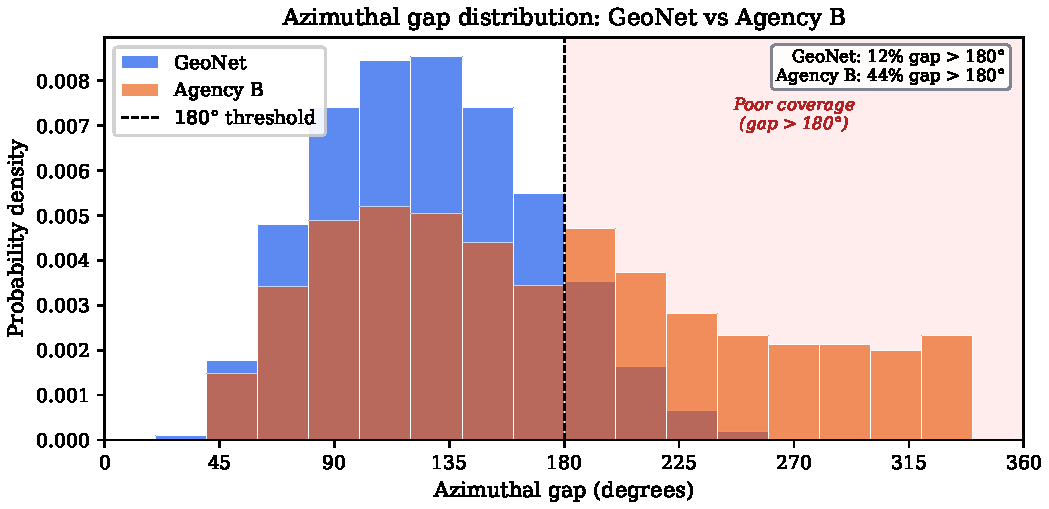
\includegraphics[width=\linewidth]{figures/fig1_azimuthal_gap.pdf}
  \caption{%
    Distribution of azimuthal gap (in degrees) for the GeoNet catalogue
    (blue) and Agency~B (orange) before merging.  The long tail
    $> 180^{\circ}$ in Agency~B reflects limited offshore station coverage.
    Events with gap $> 180^{\circ}$ receive $Q_{\text{gap}} < 10$ and a
    quality grade of D or~F.  The shaded region marks the poor-coverage
    zone.  Percentages shown are fraction of events in each catalogue with
    gap exceeding $180^{\circ}$.
  }
  \label{fig:gap}
\end{figure}

\begin{figure}[ht]
  \centering
  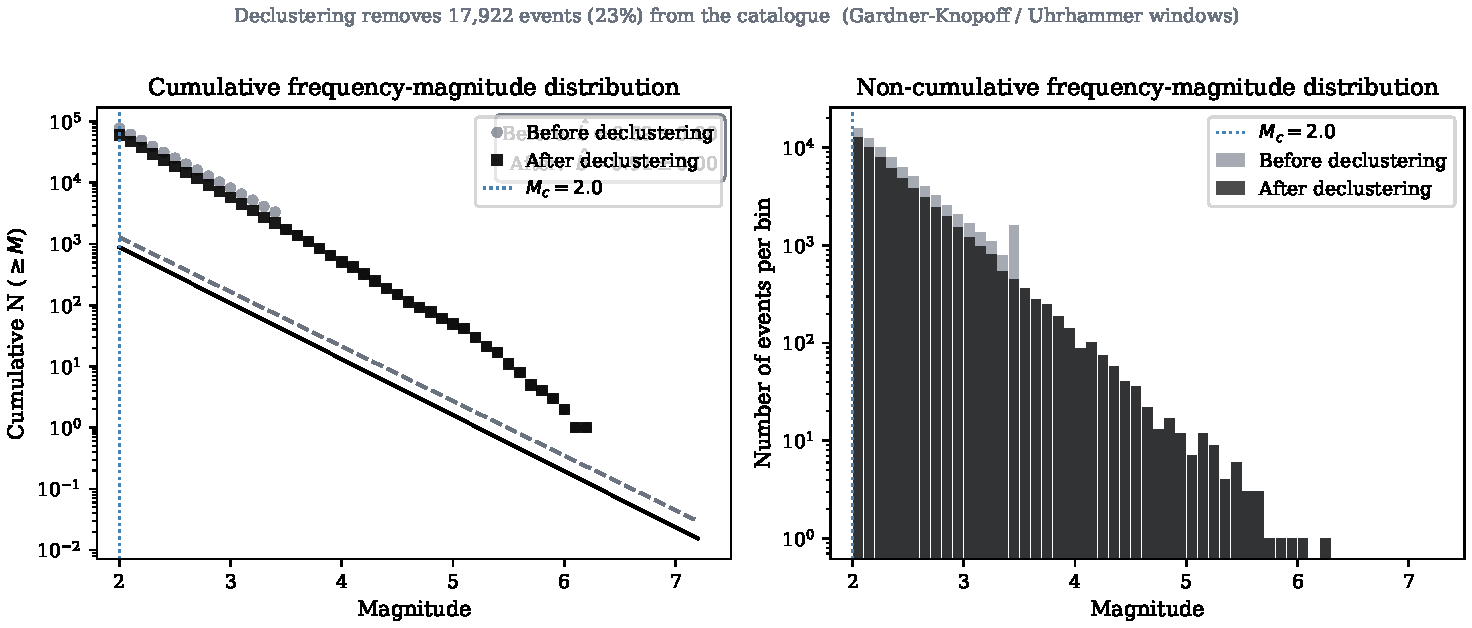
\includegraphics[width=\linewidth]{figures/fig2_fmd_declustering.pdf}
  \caption{%
    Frequency-magnitude distributions (FMD) for the synthetic New Zealand
    catalogue before (grey symbols/bars) and after (black) Gardner-Knopoff
    declustering.  \textit{Left:} cumulative FMD with maximum-likelihood GR
    fits (dashed line: before; solid line: after) above $M_c = 2.0$ (blue
    dotted line).  \textit{Right:} non-cumulative FMD showing the excess of
    small events contributed by aftershock sequences.  Declustering shifts
    $\hat{b}$ from $0.94 \pm 0.03$ to $1.02 \pm 0.03$ and removes 23\% of
    events.  Data are synthetic and for illustration only (see
    Section~\ref{sec:example}).
  }
  \label{fig:fmd}
\end{figure}

\begin{figure}[ht]
  \centering
  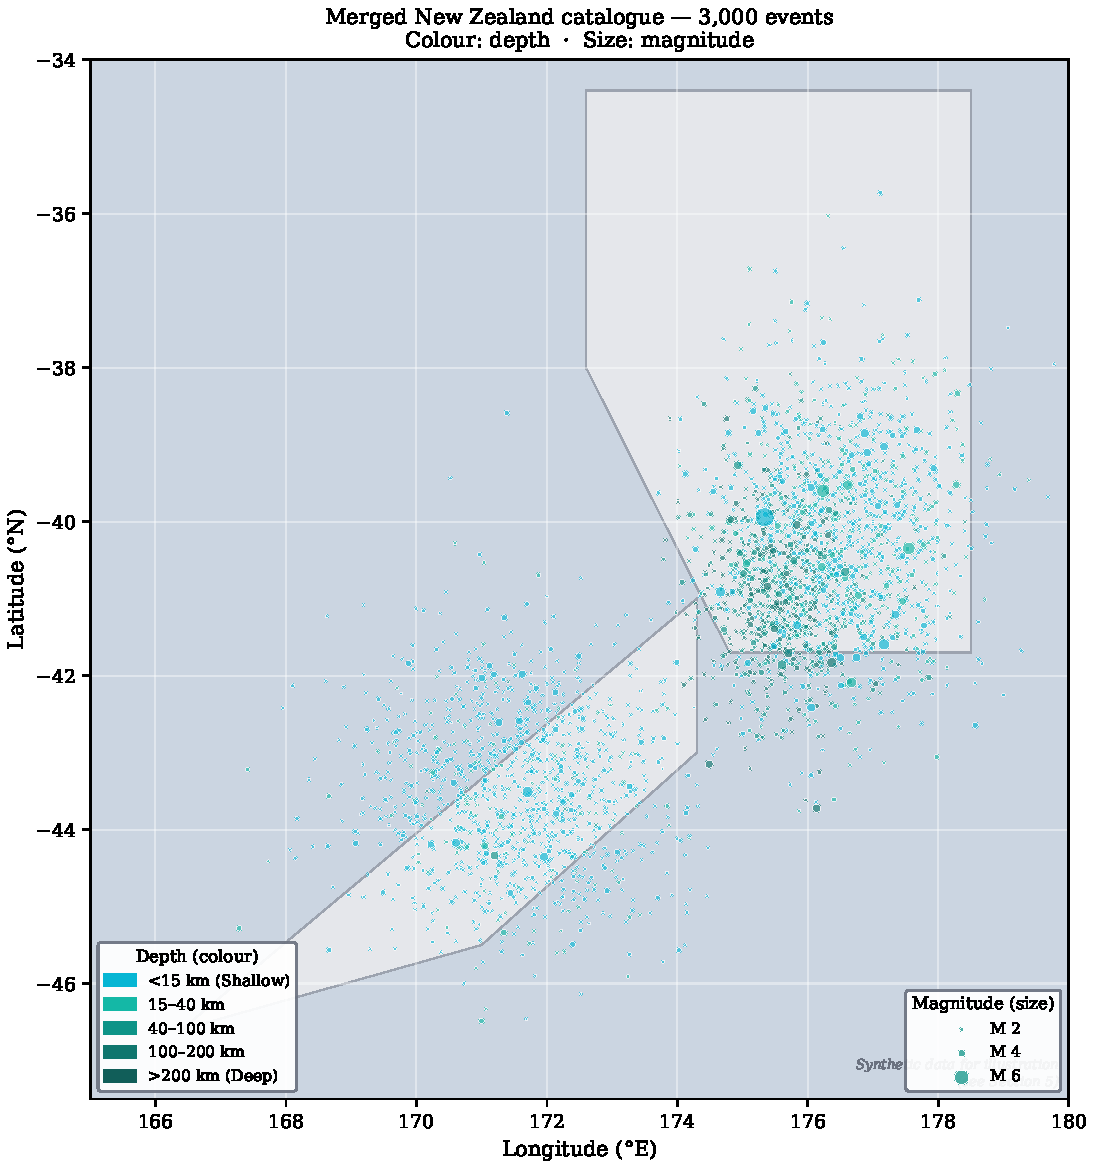
\includegraphics[width=0.82\linewidth]{figures/fig3_map.pdf}
  \caption{%
    Synthetic New Zealand seismicity map illustrating the CofC map view.
    Circle colour encodes focal depth (cyan: $<15$~km; dark teal:
    $>200$~km), matching the depth palette used in the web application.
    Circle radius scales with magnitude.  The Hikurangi subduction margin
    (offshore North Island, northeast) shows predominantly shallow seismicity;
    the central North Island cluster captures deep slab events
    ($\sim 100$~km); the South Island cluster represents Alpine Fault
    seismicity.  Data are synthetic and for illustration only.
  }
  \label{fig:map}
\end{figure}

\end{document}
